\chapter{Deployment}

The application in this research has been development using Microsoft's Mixed Reality Toolkit and has followed the platforms best practices and recommendations, thus, any issues arising when going through the following section should be answered in Microsoft's \href{https://docs.microsoft.com/en-us/windows/mixed-reality/mrtk-unity}{MRTK documentation}. The deployment process for HoloLens devices are based on sideloading of the application compiled and built with Visual Studio Community 2019, this is the standard way of both building and deploying for HoloLens. For Android the principle of sideloading is also used, but here Unity is responsible for compilation and the build process. 
The application as 


\section{Installation of Nevrolens}

This section will be a guide for installing Nevrolens on HoloLens 2 and Android from packages hosted on GitLab.
By following the instructions for HoloLens 2, this should also work for HoloLens 1, but has limited testing on that platform as it was not a focus of this research.

\subsubsection{Deploy to HoloLens 2}

\begin{enumerate}
    \item {
        \textbf{Go to the release page}\\
        Found here: \url{https://gitlab.stud.idi.ntnu.no/olevra/nevrolens/-/releases}
    }
    \item {
        \textbf{Choose a release}\\
        Preferably the topmost and latest. This research ends on is version 0.3.3. 
    }

    \item {
        \textbf{Download the HoloLens zip package}\\
        Under \textit{Packages} click on the package for HoloLens (1 and 2) to download it.
    }

    \item {
        \textbf{Unzip file}\\
        Open the downloaded ZIP-file and extract it.
    }

    \item {
        \textbf{Open the Windows Device Portal for HoloLens}\\
        Guide by Microsoft: \href{https://docs.microsoft.com/en-us/windows/mixed-reality/develop/platform-capabilities-and-apis/using-the-windows-device-portal}{Using the Windows Device Portal}
    }
    \item {
        \textbf{Install appxbundle}\\
        Under \textit{Views / Apps} click \texttt{Choose File} and locate the APPXBUNDLE-file inside the folder extracted from the ZIP-file. Then click \texttt{Install}.
    }

\end{enumerate}

\subsubsection{Deploy to Android}

\begin{enumerate}
    \item {
        \textbf{Go to the release page on your Android device}\\
        Found here: \url{https://gitlab.stud.idi.ntnu.no/olevra/nevrolens/-/releases}
    }
    \item {
        \textbf{Choose a release}\\
        Preferably the topmost and latest. This research ends on is version 0.3.3. 
    }

    \item {
        \textbf{Download the Android APK-file}\\
        Under \textit{Packages} click on the package for Android to download it.
    }

    \item {
        \textbf{Open the downloaded file.}\\
        Your device will ask for your permission to install an application from a unknown source. Accepting this, the device will start installing the application.
    }

\end{enumerate}

\section[Project Setup]{Getting started with developing the project}
This section will briefly explain how to set up the project for development, this differs from deployment in that the goal is to be able to continue development of the project from within Unity and with supporting tools. This is the process the current developer uses when developing from a new computer.
Having completed this set up deployment of the application can be done, directly from Unity for Android and through Visual Studio 2019 for HoloLens devices.


\textbf{Requirements}
\begin{enumerate}
    \item Git and Git LFS
    \item { Unity 2019.4 LTS \\
    When installing add: \textit{Android Build support} }
    \item {Visual Studio 2019 (Community or other)\\
    When installing add: \textit{Universal Windows Platform development}, \textit{USB Device Connectivity}, \textit{Game development with Unity} }
\end{enumerate}

Type the following commands in to the \textit{Git Bash}, it will clone the repository, and download all files which are to large for git with \textit{Git LFS}.
\begin{lstlisting}[numbers=none]
$ git clone "https://gitlab.stud.idi.ntnu.no/olevra/nevrolens.git"
$ cd nevrolens
$ git lfs install
$ git lfs fetch --all
\end{lstlisting}

\begin{wrapfigure}{r}{0.35\textwidth} 
    \centering
    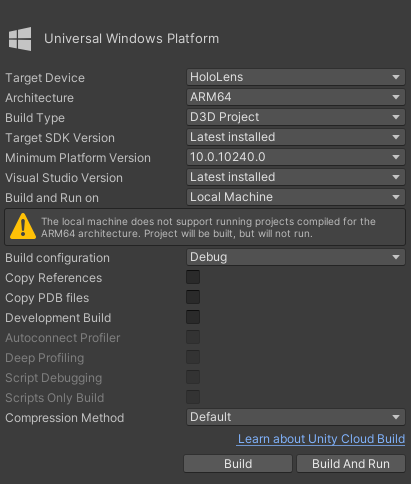
\includegraphics[width=0.35\textwidth]{fig/unitybuildhololens.png}
    \caption{Unity build configurations for HoloLens 2.}
    \label{fig:unitybuildhololens}
\end{wrapfigure}
When this has completed, open Unity Hub and locate and add the \texttt{nevrolens} repository just cloned as a Unity project. Open it with Unity 2019.4, it is critical that this version is used for MRTK to work properly. First time opening this project will take some time, when it is done the project is ready. Deployment for HoloLens 2 can be done by building (ctrl+shift+b) the Unity project with the configurations in \autoref{fig:unitybuildhololens} and opening the outputted \texttt{Nevrolens.sln} solution in Visual Studio 2019 and running the solution for \texttt{Remote Machine} while the HoloLens 2 device is connected by USB. Refer to the MRTK documentation for OTA deployment through Wi-Fi. Android deployment is done by simply choosing Android in Unity's build configuration view and clicking \textit{Build And Run} while the Android device is connected by USB and is set to developer mode. Make sure to follow the MRTK documentation on which version of ARCore etc. that should be installed in the project, found \href{https://microsoft.github.io/MixedRealityToolkit-Unity/version/releases/2.5.1/Documentation/CrossPlatform/UsingARFoundation.html}{here}.
% The deployment process can be found in MRTK documentation 